\documentclass[border=10pt]{standalone}
\usepackage{pgfplots}
\pgfplotsset{compat=1.18}
\begin{document}
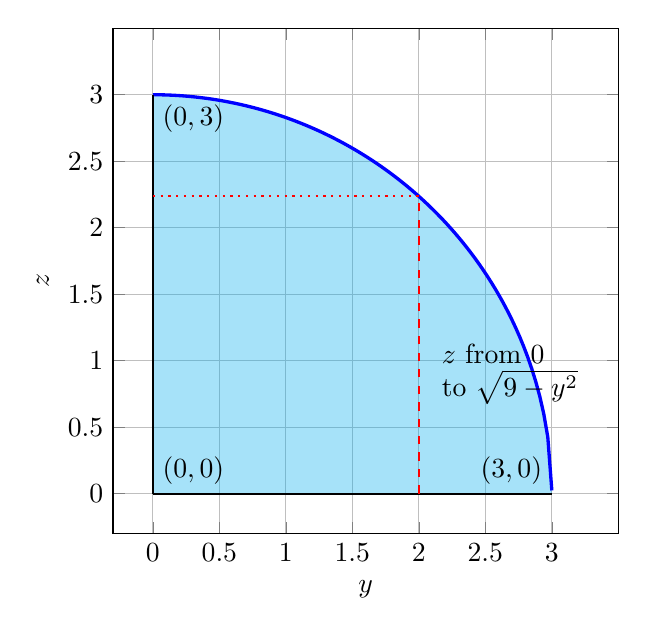
\begin{tikzpicture}
\begin{axis}[
    axis lines=box,
    xlabel=$y$, ylabel=$z$,
    xmin=-0.3, xmax=3.5,
    ymin=-0.3, ymax=3.5,
    width=8cm, height=8cm,
    grid=major,
    enlargelimits=false,
    xtick={0,0.5,1,1.5,2,2.5,3},
    ytick={0,0.5,1,1.5,2,2.5,3},
]
% shaded quarter disk
\addplot[fill=cyan, opacity=0.35, draw=none, domain=0:3, samples=100]
    {sqrt(9-x^2)} \closedcycle;
% circle arc
\addplot[blue, very thick, domain=0:3, samples=100] {sqrt(9-x^2)};
% axes
\addplot[black, thick] coordinates {(0,0) (3,0)};
\addplot[black, thick] coordinates {(0,0) (0,3)};
% typical strip at y = 2
\addplot[red, thick, dashed] coordinates {(2,0) (2,{sqrt(5)})};
\addplot[red, dotted, thick] coordinates {(0,{sqrt(5)}) (2,{sqrt(5)})};
\node[right, align=left] at (axis cs:2.10,0.9)
    {$z$ from $0$\\ to $\sqrt{9-y^2}$};
% vertices
\node[above right] at (axis cs:0,0) {$(0,0)$};
\node[above left] at (axis cs:3,0) {$(3,0)$};
\node[below right] at (axis cs:0,3) {$(0,3)$};
\end{axis}
\end{tikzpicture}
\end{document}
